% !TEX root = catron-dissertation.tex
\epstopdfsetup{outdir=./images/02_background/}

\chapter{Literature Review}
\label{chap:02_lit_review}

Strong narrow-band acoustic waves traveling upstream have been measured in-flight with optical wavefronts from a turret as part of the AAOL program \cite{DeLucca-2018-gBQdjTmT}.
This was one of the first indications that a temporally narrow-band acoustic signal related to a fan was a noise source that could contribute significantly to the overall signal.
Additional measurements have shown both narrow-band and broad-band acoustic signals measured in-flight through a flat window with both boundary and shear layers present \cite{Gordeyev-2020-6HnfJMnC}.
Broad-band acoustic signals have been reported previously in optical wavefront measurements during boundary layer measurements in wind-tunnels but the effect was only  important at low temporal frequencies \cite{Gordeyev-2014-jcJndkHM,Smith-2013-VXArwwux}.
Optical measurements have also been made looking specifically for the acoustic waves inside a wind-tunnel, by looking for narrow-band optical disturbances associated with the wind-tunnel fan, with various model support structures \cite{Catron-2018-DdVp6VZf}, or with acoustic duct modes, showing that the optical disturbances due to the acoustic environment not only travel upstream at $u-c$, but also downstream at $u+c$ and cross-stream at $\pm c$ \cite{Catron-2020-x8njYmmu}.

The literature review will consist of primarily two sections.
The first section will examine aero-optics while the second will look at acoustics inside of ducts.

\section{Aero-Optics}
In optically active flows the index-of-refraction, $n$, varies locally along with other fluid properties.
Gladstone and Dale \cite{Gladstone-1863-ND4wtDT9} found that the index-of-refraction is primarily a function of density with a loose dependence on the wavelength of light.
Gladstone and Dale proposed a ``specific refractive energy'' now known as the Gladstone-Dale constant, $K_{GD}$,
\begin{equation}
  K_{GD} = \frac{n-1}{\rho}\textrm{.}
  \label{eqn:02_gladstone_dale_constant}
\end{equation}
For air the refractive index can be related to state quantities \cite{Valley-1965-F3k3cmv6}
\begin{equation}
  n-1 = 77.6\times 10^{-6}\frac{p}{T}\left(1+\frac{7.53\times10^{-3}}{\lambda^2}\right)\textrm{,}
  \label{eqn:02_refractive_index_ptlambda}
\end{equation}
where $p$ is in mbar, $T$ is in K, and $\lambda$ is in $\mu$m.
By combining this relationship with the ideal gas law, the Gladstone-Dale constant can be determined as a function of light wavelength,
\begin{equation}
  K_{GD} = 2.23\times10^{-4}\left(1+\frac{7.53\times10^{-3}}{\lambda_{\mu m}^2}\right) \: \left[\frac{m^3}{kg}\right]\textrm{.}
  \label{eqn:02_gladstone_dale_wavelength}
\end{equation}
The Gladstone-Dale constant for air over the visible range is shown in Figure \ref{fig:02_gladstone_dale_wavelength}.
\begin{figure}
  \centering
  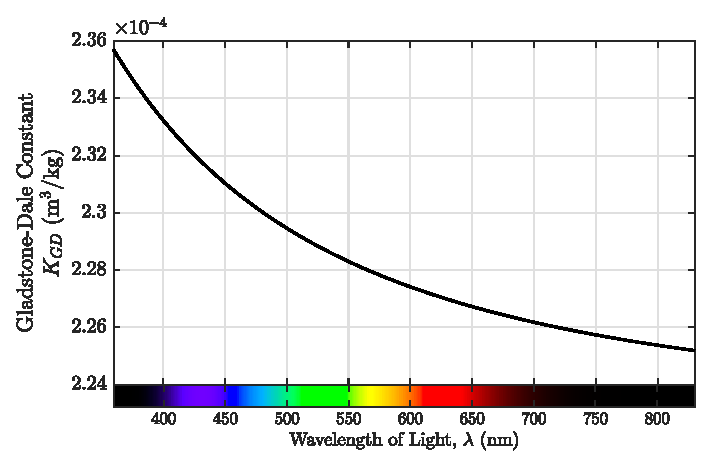
\includegraphics{../matlab/02_background/gladstone_dale_wavelength.eps}
  \caption{Gladstone-Dale constant for air over the visible wavelength range.}
  \label{fig:02_gladstone_dale_wavelength}
\end{figure}
While the value for $K_{GD}$ does vary over the visible range, it is only a few percent, and many sources use an average value of 2.27$\times10^{-4}$ m$^3$/kg for the visible and near-infrared \cite{Gardiner-1980-reW8xrCb}.
The Gladstone-Dale relationship is typically presented as
\begin{equation}
  n = 1+K_{GD}\rho
  \label{eqn:02_gladstone_dale_relation}
\end{equation}
but when applied to situations where there are significant fluctuations in the flow an alternate form is often more useful
\begin{equation}
  n'=K_{GD}\rho'
  \label{eqn:02_gladstone_dale_relation_fluctuating}
\end{equation}
where $'$ denotes the fluctuating component ($n' = n-\bar{n}$).

When a beam with an initially planar wave front passes through a region of optically active flow its wavefront becomes aberrated.
The optical path length ($\opl$) at any point in the beam can be obtained by integrating the index of refraction along the propagation of an optical ray \cite{Klein-1986-8Vx29RfE}.
\begin{equation}
  \opl (x,y,t) = \int^{s_2}_{s_1} n(x,y,z,t)ds
  \label{eqn:02_opl}
\end{equation}
The optical path difference ($\opd$), is then the spatially-averaged $\textrm{OPL}$ over an aperture removed from the OPL.
\begin{equation}
  \opd(x,y,t) = \opl(x,y,t)-\langle\opl(x,y,t)\rangle
  \label{eqn:02_opd}
\end{equation}
When working with fluctuating components, the $\opd$ can be calculated directly
\begin{equation}
  \opd(x,y,t) = \int^{s_2}_{s_1} n'(x,y,z,t)ds \textrm{.}
  \label{eqn:02_opd_n}
\end{equation}

As a finite beam of light travels normal to its wavefront it is diffracted, producing a theoretical limit on the performance of an optical system, i.e. diffraction-limited \cite{Born-1965-HHGYgjdH}.
Sommerfeld defined diffraction as ``any deviation of light rays from rectilinear paths which cannot be interpreted as reflection or refraction'' \cite{Sommerfeld-1954-ep2AWrFF}.
Diffraction through an aperture can be approximated with the Huygens-Fresnel principle by assuming that every point within the aperture produces a spherical wavelet \cite{Huygens-1690-gD8nxCn8},
\begin{equation}
  U(x_0,y_0) = \iint_{Ap} h(x_0,y_0;x_1,y_1)U(x_1,y_1)dx_1dy_1 \textrm{,}
  \label{eqn:02_huygens}
\end{equation}
where $U$ is the complex amplitude, the subscripts 0 and 1 represent the coordinates of the observation plane and aperture plane respectively, and
\begin{equation}
  h(x_0,y_0;x_1,y_1) = \frac{1}{j\lambda}\frac{\exp\{jkr_{01}\}}{r_{01}}\cos(\overrightarrow{n},\overrightarrow{r}_{01}) \textrm{,}
  \label{eqn:02_huygens_h}
\end{equation}
where $r_{01} = \sqrt{z^2+(x_0-x_1)^2+(x_0-y_1)^2}$, is the distance between any point in the observation and aperture planes.
Equation \ref{eqn:02_huygens} can be expanded to infinite limits of integration with the Kirchhoff boundary conditions where $U(x_1,y_1)$ is equal to zero outside of the aperture.
The obliquity factor, $\cos(\overrightarrow{n},\overrightarrow{r}_{01})$, can be approximated as being equal to one by assuming that the observation plane is at a much greater distance than the size of the aperture and is a small finite region.
The accuracy of this assumption is with 5\% if the angle between  $\overrightarrow{n}$ and $\overrightarrow{r}_{01}$ does not exceed $18^\circ$\cite{Goodman-1968-zPUmuuzx}.
With this assumption and for similar accuracy, $r_{01}$ in the denominator of Equation \ref{eqn:02_huygens_h} can be replaced with $z$, resulting in
\begin{equation}
  h(x_0,y_0;x_1,y_1) \approxeq \frac{1}{j\lambda z}\exp\{jkr_{01}\} \textrm{.}
\end{equation}

The Fresnel approximation replaces the spherical wavelets with a quadratic surface \cite{Fresnel-1818-FmMCMbDK},
\begin{equation}
  h(x_0,y_0;x_1,y_1) = \frac{\exp\{jkz\}}{j\lambda z}\exp\left\{j\frac{k}{2z}[(x_0-x_1)^2+(y_0-y_1)^2]\right\} \textrm{,}
  \label{eqn:02_fresnel_approx}
\end{equation}
which has a theoretical requirement that $z^3 \gg \frac{\pi}{4\lambda}\max\{[(x_0-x_1)^2+(y_0-y_1)^2]^2\}$ due to the limited number of terms used in a binomial expansion of $r_{01}$.
In practice this limit is not that critical \cite{Goodman-1968-zPUmuuzx}.
By combining Equations \ref{eqn:02_fraunhofer} and \ref{eqn:02_fresnel_approx}, an expression for Fresnel diffraction can be obtained,
\begin{equation}
  \begin{aligned}
    U(x_0,y_0) =& \frac{\exp\{jkz\}}{j\lambda z}\exp\left\{j\frac{k}{2z}(x_0^2+y_0^2)\right\}\iint_{-\infty}^{+\infty}\left[U(x_1,y_1)\exp\left\{j\frac{k}{2z}(x_1^2+y_1^2)\right\}\right] \\
    &\exp\left\{-j\frac{2\pi}{\lambda z}(x_0x_1+y_0y_1)\right\} dx_1dy_1 \textrm{.}
  \end{aligned}
  \label{eqn:02_fresnel}
\end{equation}
The function $U(x_0,y_0)$ may therefore be found from a two-dimensional Fourier transform:
\begin{equation}
  U(x_0,y_0) = \ft_2\left[U(x_1,y_1)\exp\left\{j\frac{k}{2z}(x_1^2+y_1^2)\right\}\right]
  \label{eqn:02_fresnel_fft}
\end{equation}
where $\ft_2$ is the two-dimensional Fourier transform and transform is evaluated at the spatial frequencies $\xi_x = x_0/\lambda z$, $\xi_y = y_0/\lambda z$.

The Fraunhofer approximation \cite{Goodman-1968-zPUmuuzx},
\begin{equation}
  z \gg \frac{k\max[x_1^2+y_1^2]}{2} \textrm{,}
  \label{eqn:02_fraunhofer_approx}
\end{equation}
places further restrictions than the Fresnel assumption approximation which results in
$\exp\left\{j\frac{k}{2z}(x_1^2+y_1^2)\right\}$ being approximately unity over the aperture further simplifying Equation \ref{eqn:02_fresnel} to
\begin{equation}
  \begin{aligned}
    U(x_0,y_0) =& \frac{\exp\{jkz\}}{j\lambda z}\exp\left\{j\frac{k}{2z}(x_0^2+y_0^2)\right\} \\
    &\iint_{-\infty}^{+\infty}U(x_1,y_1)\exp\left\{-j\frac{2\pi}{\lambda z}(x_0x_1+y_0y_1)\right\} dx_1dy_1 \textrm{.}
  \end{aligned}
  \label{eqn:02_fraunhofer}
\end{equation}
Equation \ref{eqn:02_fraunhofer} known as the Fraunhofer diffraction integral.
In Fraunhofer diffraction, the function $U(x_0,y_0)$ maybe found from the Fourier transform of $U(x_1,y_1)$, when evaluated at the spatial frequencies $\xi_x = x_0/\lambda z$, $\xi_y = y_0/\lambda z$.
For additional details on the derivation of Huygens, Fresnel, and Fraunhofer diffraction, including more in depth discussion on the assumptions and limits, see Goodman \cite{Goodman-1968-zPUmuuzx}.

The optical path difference can be related to the complex amplitude by \cite{Cicchiello-1997-RHxhNMxj},
\begin{equation}
  U(x_1,y_1) = \exp\left\{j\frac{2\pi}{\lambda}\opd(x_1,y_1)\right\} \textrm{.}
\end{equation}
Using the Fraunhofer diffraction integral, the nearfield $\opd$ disturbance can therefore be used to calculate the farfield intensity profile ($I = UU^*$),
\begin{equation}
  I(x_0,y_0) = \left|\ft_2\left(\exp\left\{j\frac{2\pi}{\lambda}\opd(x_1,y_1)\right\}\right)\right|^2 \textrm{,}
\end{equation}
where the transform is evaluated at the spatial frequencies $\xi_x = x_0/\lambda z$, $\xi_y = y_0/\lambda z$ in the observation plane and the complex amplitude outside of the aperture is zero.
For cases in which optical aberrations are nonexistent (i.e. $\opd(x,y,t)=0$), the farfield irradiance pattern that results from Equation \ref{eqn:02_fraunhofer} is caused entirely by diffraction from the optical aperture, and is referred to as the ``diffraction-limited'' irradiance pattern.
For a beam with a flat wave front and circular aperture, the farfield irradiance pattern is the Airy’s disk, and the peak irradiance at the center of the disk, $I_0$ , is the maximum irradiance that can be achieved by the optical system:
\begin{equation}
  I_0 = \left(\frac{kAp^2}{8z}\right)^2
  \label{eqn:02_airy_pattern}
\end{equation}
where $k$ is the wavenumber ($k=2\pi /\lambda$), $Ap$ is the aperture diameter, and $z$ is the distance from the aperture to the observation plane.
In the presence of aero-optical aberrations, $\opd(x,y,t)$ is non-zero, and the farfield irradiance pattern in this case tends to be more spread out and diffuse than the diffraction-limited case; furthermore, the beam may be shifted off target by optical tip/tilt imposed by the aberrations.

The Strehl ratio ($\sr$), is the ratio of intensity on target ($I$) to the diffraction-limited on target intensity ($I_0$):
\begin{equation}
  \sr=\frac{I}{I_0}
  \label{eqn:02_strehl_simple}
\end{equation}
The Strehl ratio can be computed accurately by applying Equation \ref{eqn:02_fraunhofer} twice, once for the diffraction-limited case to obtain $I_0$, and a second time with the $\opd$ field due to aero-optical aberrations included to obtain $I$.
The farfield performance, can also be estimated via the Mar\'{e}chal approximation:
\begin{equation}
  \sr(t) \equiv \frac{I(t)}{I_0} \approx \exp \left\{-\left[\frac{2\pi \opdrms(t)}{\lambda}\right]^2\right\}
  \label{eqn:02_strehl_ratio}
\end{equation}
where $\opdrms$ is the spatial rms of the wave front and $\lambda$ is the wavelength of the beam.
\begin{figure}
  \centering
  \begin{subfigure}[t]{0.45\textwidth}
    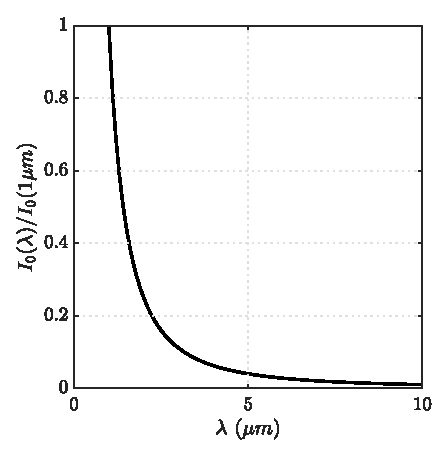
\includegraphics{../matlab/02_background/farfield_intensity.eps}
    \caption{}\label{fig:02_farfield_intensity}
  \end{subfigure}
  ~
  \begin{subfigure}[t]{0.45\textwidth}
    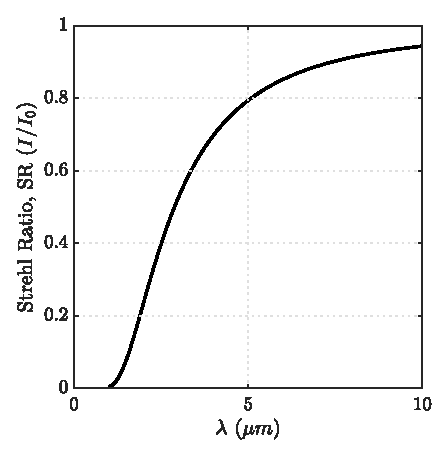
\includegraphics{../matlab/02_background/all_strehl_ratio.eps}
    \caption{}\label{fig:02_all_strehl_ratio}
  \end{subfigure}
  \caption{(\subref{fig:02_farfield_intensity}) Diffraction limited on target intensity as a function of wavelength normalized by the value at $\lambda$ = 1 $\mu$ m. (\subref{fig:02_all_strehl_ratio}) Strehl ratio as a function of wavelength for an aberration that gives SR = 0.95 at $\lambda$ = 10.6 $\mu$m.}
  % \label{FIG:airy_strehl}
\end{figure}
Equation \ref{eqn:02_strehl_ratio} reveals a key relationship between $\opd$, wavelength, and the farfield performance, plotted in Figure \ref{fig:02_all_strehl_ratio}, and shows that, for the same aero-optical aberration, the Strehl ratio decreases substantially as system wavelength decreases.
On the other hand, Equation \ref{eqn:02_airy_pattern} shows that the diffraction-limited farfield irradiance increases as the wavelength is shortened, plotted in Figure \ref{fig:02_farfield_intensity}.
Together, Figure \ref{fig:02_farfield_intensity} and \ref{fig:02_all_strehl_ratio} show that as modern optical systems move to shorter wavelengths to increase $I_0$, aero-optical aberrations cause a much more serious degradation of the Strehl ratio, illustrating why aero-optical considerations are critical in the development of new airborne optical systems.
Figure \ref{fig:02_necessary_opd} shows the $\opdrms$ necessary to achieve various Strehl ratios over a range of wavelengths.
\begin{figure}
  \centering
  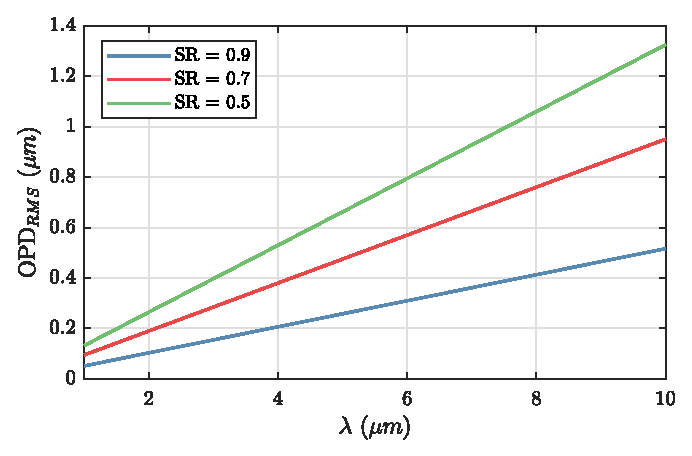
\includegraphics{../matlab/02_background/necessary_opd.eps}
  \caption{$\opdrms$ values necessary to obtain Strehl ratios of 0.9, 0.7, and 0.5 over a range of wavelengths.}
  \label{fig:02_necessary_opd}
\end{figure}
As the wavelength of light decreases the required $\opdrms$ decreases linearly for a fixed Strehl ratio.


\subsection{Typical Optical Wavefront Measurement System}
A diagram of a typical double-pass Shack-Hartmann wavefront front sensor setup is shown in Figure \ref{fig:02_typical_wavefront_system}.
\begin{figure}
  \centering
  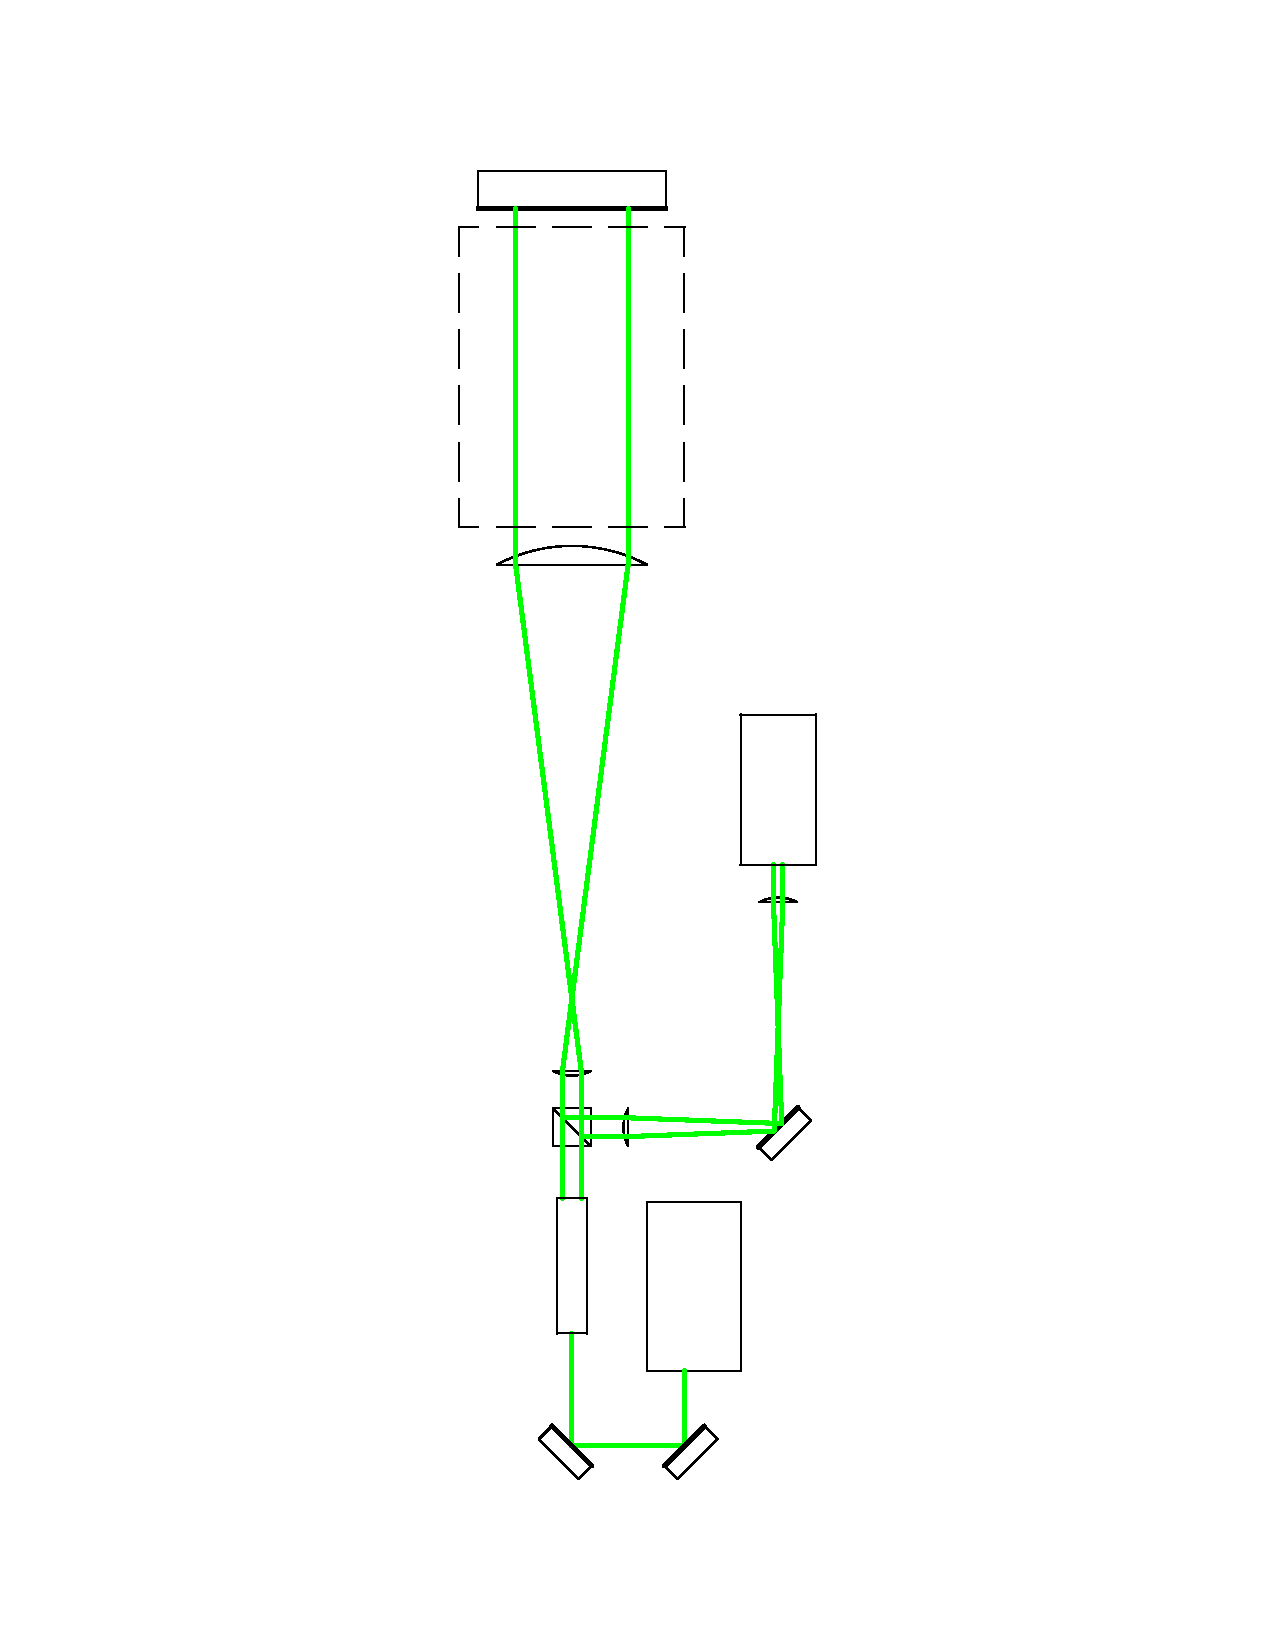
\includegraphics[width=3.25in,clip,trim=170 75 170 75]{../cad/wavefront_setup.pdf}
  \put(-72,62){\rotatebox{90}{\Large LASER}}
  \put(-145,78){\rotatebox{90}{BEAM}}
  \put(-135,65){\rotatebox{90}{EXPANDER}}
  \put(-150,200){\rotatebox{90}{\Large PRIMARY TELESCOPE}}
  \put(-130,405){\rotatebox{90}{\Large MEASUREMENT}}
  \put(-112,432){\rotatebox{90}{\Large REGION}}
  \put(-95,160){\rotatebox{60}{\Large REIMAGING}}
  \put(-80,155){\rotatebox{60}{\Large TELESCOPE}}
  \put(-10,245){\rotatebox{90}{\Large WAVEFRONT}}
  \put(5,260){\rotatebox{90}{\Large SENSOR}}
  \put(-59,441){\fcolorbox{white}{white}{\Large $\gamma$}}
  \put(-90,480){\fcolorbox{white}{white}{\Large $\Longleftarrow$ Flow Direction}}
  \caption{Typical double-pass optical wavefront measurement setup.}
  \label{fig:02_typical_wavefront_system}
\end{figure}
The system starts with the laser in the bottom of the plot, which is then expanded to a larger diameter.
The beam expander used in this research increased the diameter of the beam to approximately 1-inch.
The larger diameter beam then passes through a beam splitter where half of the intensity is discarded and the other half proceeds to the primary telescope.
The primary telescope expands the beam to the desired size for the first passage through the measurement region.
For measurements made in a wind-tunnel, the beam angle, $\gamma$, is typically defined based on the flow direction \cite{Gordeyev-2014-jcJndkHM} with $0^\circ$ being looking straight into the flow and $180^\circ$ looking downstream.

A large mirror is used to return the beam along the same path for a second passage through the measurement region where the primary telescope shrinks the beam back down to a 1-inch diameter.
On the return path, the beam splitter sends half of the intensity back through the beam expander to the laser and half to the reimaging telescope.
The reimaging telescope serves two purposes, the first is to create an image plane for the wavefront sensor at the desired object plane location, typically the return mirror for a double-pass setup.
The second is to reduce the beam diameter for the wavefront sensor to a size that depends on the resolution and frame rate needed for a measurement.

The Shack-Hartmann wavefront sensor is comprised of a lenslet array and a camera \cite{Geary-1995-TQXWWFW2}.
A diagram of how the wavefront sensor functions can be seen in Figure \ref{fig:02_lenslet_array}.
\begin{figure}
  \centering
  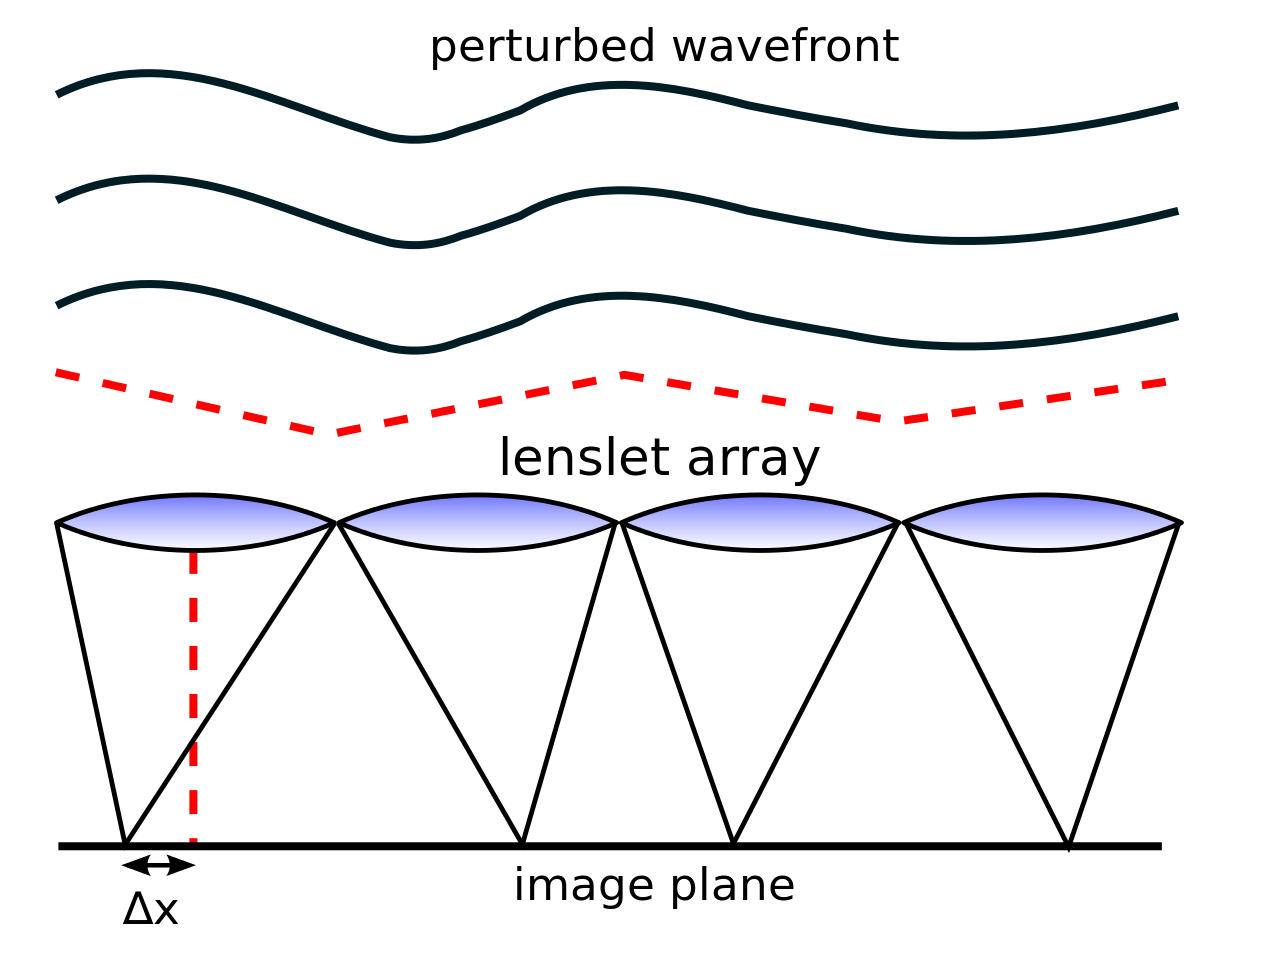
\includegraphics[width=0.8\textwidth]{../other-sources/Shack_Hartmann_WFS_lensletarray.png}
  \caption{Diagram of a Shack-Hartmann wavefront sensor comprised of four lenslets. The black line represents the perturbed wavefront and the red line the mean slope over each lenslet. The focal point of the wavefront is shifted by $\Delta x$ from the center-line of the lenslet based on the mean slope of the wavefront. \cite{Shack-Hartman-Diagram-Wikipedia}}
  \label{fig:02_lenslet_array}
\end{figure}
The perturbed wavefront is represented by the black lines on the top of the figure.
Each lenslet produces a focused spot on the image plane with a location given by the average slope of the portion of the wavefront that passes through the lenslet.
By measuring the displacement, \cite{Nightingale-2013-gqr4p7GY}, of the focal dot from its normal position, the average slope, $\theta_x$ and $\theta_y$, of the wavefront over a lenslet can be measured,
\begin{equation}
  \theta_x = \tan^{-1}{\frac{\Delta x}{f}} \approx\frac{\Delta x}{f} \textrm{,}
\end{equation}
where $f$ is the focal length of the lenslet.
With an array of gradient data, the optical path difference at each lenslet can be calculated using a number of integration methods \cite{Huang-2015-W29DqPyp}, for example, one well-known method is the Southwell method \cite{Southwell-1980-KqUZMXRB}.

\subsection{Boundary Layer Optical Distortions}
Because optical wavefront measurements within a wind tunnel will usually include the optical distortion from the boundary layer(s) on the wind-tunnel wall(s), it is important to have some familiarity.
The time-averaged optical disturbance for a large aperture has been reported as,
\begin{equation}
  \opdrms = B(\gamma)K_{GD}\rho_\infty M^2\delta\sqrt{C_f}G(M) \textrm{,}
  \label{eqn:02_opdrms_gor}
\end{equation}
where $C_f$ is the skin-friction coefficient.
The function $B(\gamma)$ accounts for angle between the beam and the direction of flow, $\gamma$:
\begin{equation}
  B(\gamma) = \frac{0.19}{\sin(\gamma)} \textrm{,}
\end{equation}
and
\begin{equation}
  G(M) = 1-0.19M^2+0.03M^4 \textrm{.}
\end{equation}
Aperture size can be accounted for by Figure \ref{fig:02_gordeyev_2014} (Figure 18 in Gordeyev \cite{Gordeyev-2014-jcJndkHM}) with an approximation for the fit,
\begin{equation}
  \frac{\opdrms(Ap)}{\opdrms} \approx 1-a\exp\left\{b\frac{Ap}{\delta}\right\}-(1-a)\exp\left\{c\frac{Ap}{\delta}\right\} \textrm{,}
  \label{eqn:02_opdrms_gor_fit}
\end{equation}
where $a=0.7795$, $b=-0.9616$, and $c=-0.1382$.
\begin{figure}
  \centering
  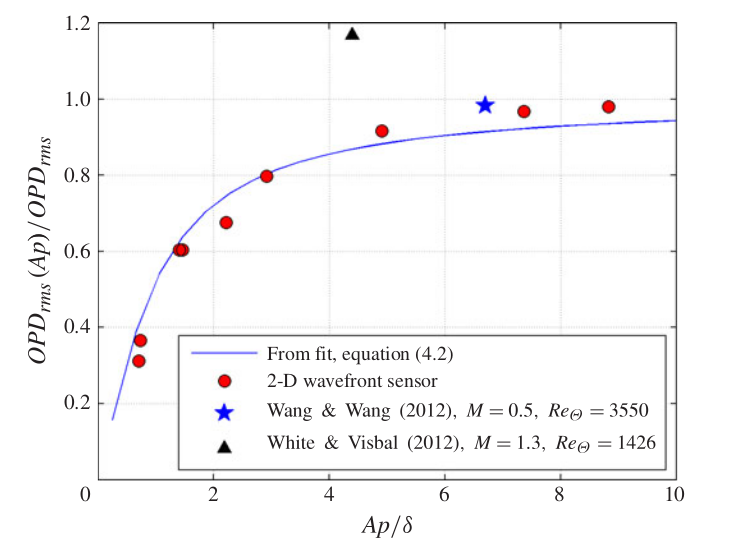
\includegraphics[width=0.75\textwidth]{../other-sources/gordeyev_2014_figure_18.png}
  \caption{Aperture size correction for $\opdrms$ (Figure 18 in Gordeyev \cite{Gordeyev-2014-jcJndkHM}).}
  \label{fig:02_gordeyev_2014}
\end{figure}

\section{Duct Acoustics}
This section will look at acoustics when confined to a duct in which the acoustic waves primarily travel in the direction of one axis and have walls confining the acoustics along the other two axes as is the case inside of a wind tunnel.
Figure \ref{fig:02_duct_drawing} shows the diagram used for deriving the acoustic properties inside of a constant area duct.
\begin{figure}
\centering
    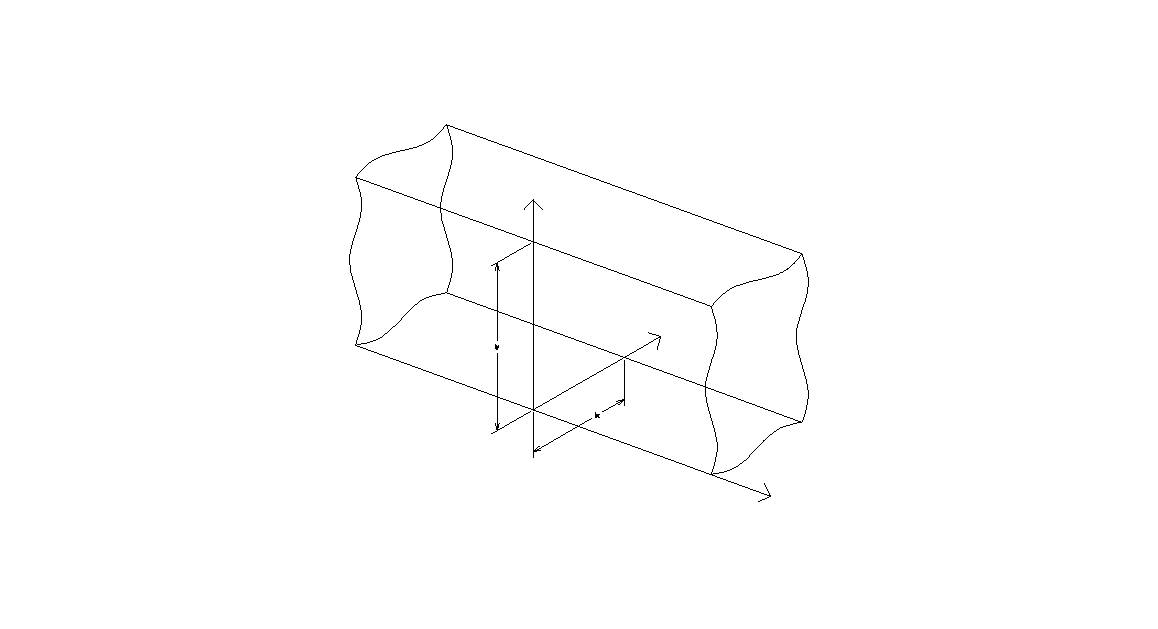
\includegraphics[trim=2.2in 0.7in 2.2in 0.7in,clip,width=4.5in]{../autocad/02_background/duct_drawing.eps}
    \put(-155,62){\fcolorbox{white}{white}{$l_x$}}
    \put(-227,113){\fcolorbox{white}{white}{$l_y$}}
    \put(-103,119){$\mathbf{x}$}
    \put(-198,220){$\mathbf{y}$}
    \put(-26,4){$\mathbf{z}$}
  \caption{Duct with a rectangular cross-section.}
  \label{fig:02_duct_drawing}
\end{figure}

The derivation presented here is primarily influenced by Munjal \cite{Munjal-2014-w28y4EyP} along with Jacobsen and Juhl \cite{Jacobsen-2013-PHD3v3YZ}.
The assumption used in this derivation is that the duct is of constant cross-section;
methods used to solve for the acoustic field in a wind tunnel with varying flow cross sections are presented later in Section \ref{sect:03_test_section}.
This means that all mean quantities ($\rho_0$, $\mathbf{u_0}$, ...) are constant throughout space and time.
Starting with the linearized inviscid forms of the conservation of mass,
\begin{equation}
  \frac{\mathbf{D}\rho}{\mathbf{Dt}} + \rho_0\nabla\cdot\mathbf{u} = 0 \textrm{,}
  % \frac{\partial\rho}{\partial t} + \mathbf{u}\cdot\nabla\rho + \rho_0(\nabla\cdot\mathbf{u}) = 0 \textrm{,}
  \label{eqn:02_cons_mass}
\end{equation}
and conservation of momentum,
\begin{equation}
  \rho_0\frac{\mathbf{Du}}{\mathbf{Dt}} + \nabla p = 0 \textrm{.}
  % \rho_0\frac{\partial\mathbf{u}}{\partial t} + \rho_0(\mathbf{u_0}\cdot\nabla)\mathbf{u} + \nabla p = 0 \textrm{.}
  \label{eqn:02_cons_mom}
\end{equation}
The definition of the speed of sound ($\left.\frac{\partial p}{\partial\rho}\right|_s = c_0^2$) is then substituted into Equation \ref{eqn:02_cons_mass},
\begin{equation}
  \frac{1}{c_0^2}\frac{\mathbf{D}p}{\mathbf{Dt}} + \rho_0\nabla\cdot\mathbf{u} = 0 \textrm{,}
  % \frac{1}{c_0^2}\frac{\partial p}{\partial t} + \frac{1}{c_0^2}(\mathbf{u}\cdot\nabla p) + \rho_0(\nabla\cdot\mathbf{u}) = 0 \textrm{,}
  \label{eqn:02_cons_mass_p}
\end{equation}
where $c_0$ is the speed of sound at average fluid properties ($\rho_0$, $p_0$, $T_0$, ...).
Next the difference between the material derivative ($\mathbf{D}/\mathbf{Dt}$) of Equation \ref{eqn:02_cons_mass_p} and the partial derivative ($\partial/\partial\mathbf{x}$) of Equation \ref{eqn:02_cons_mom} with respect to space is taken which results in the convected 3-D wave equation,
\begin{equation}
  \left(\frac{\mathbf{D}^2}{\mathbf{Dt}^2}-c_0^2\nabla^2\right)p=0\textrm{.}
  \label{eqn:02_wave_conv_3_c}
\end{equation}
Expanding the material derivative and dividing by $c_0^2$,
\begin{equation}
  \left(\frac{1}{c_0^2}\frac{\partial^2}{\partial t^2} + \frac{2\mathbf{M}}{c_0}\frac{\partial^2}{\partial t\partial\mathbf{x}} - (1-\mathbf{M}^2)\nabla^2\right)p = 0 \textrm{,}
  \label{eqn:02_wave_conv_expand}
\end{equation}
where $\mathbf{M} = \mathbf{u_0}/c_0$.
By using the fact that $c_0=\omega/k_0$, Equation \ref{eqn:02_wave_conv_3_c} can be written in a more convent form,
\begin{equation}
  \left(\frac{1}{\omega^2}\frac{\partial^2}{\partial t^2} + \frac{2\mathbf{M}}{\omega k_0}\frac{\partial^2}{\partial t\partial\mathbf{x}} - \frac{1-\mathbf{M}^2}{k_0^2}\nabla^2\right)p = 0 \textrm{,}
  \label{eqn:02_wave_conv_3}
\end{equation}
where $\omega$ is the angular frequency and $k_0$ is the total wavenumber.

At this point the pressure field is written in complex form and assumed to be separable in both time and space such that $\hat{p}(\mathbf{x},t) = \hat{p}(x,y)\hat{p}(z)\hat{p}(t)$.
The temporal solution is assumed to take the form
\begin{equation}
  \hat{p}(t) = \exp\left\{j\omega t\right\} \textrm{,}
  \label{eqn:02_pressure_solution_time}
\end{equation}
which results in the spatial component of the convecting wave equation
\begin{equation}
  \left((1-\mathbf{M}^2)\nabla^2-2jk_0\mathbf{M}\nabla+k_0^2\right)\hat{p}(x,y)\hat{p}(z) = 0 \textrm{.}
  \label{eqn:02_wave_conv_space}
\end{equation}
This can be further split into axial and cross-sectional components by splitting $k_0$ into components,
\begin{equation}
  k_0 = \sqrt{k_{xy}^2+k_z^2} \textrm{,}
  \label{eqn:02_k0}
\end{equation}
and because the mean flow is only in the axial direction ($\mathbf{M} = M\mathbf{\hat{k}}$).
The cross-sectional component is a typical Helmholtz equation
\begin{equation}
  \left(\frac{\partial^2}{\partial x^2}+\frac{\partial^2}{\partial y^2}\right)\hat{p}_{xy}(x,y)+k_{xy}^2\hat{p}(x,y) = 0 \textrm{,}
  \label{eqn:02_wave_xy}
\end{equation}
whose solution,
\begin{equation}
  \hat{p}(x,y) = \Psi_m(x,y) \textrm{,}
  \label{eqn:02_pressure_solution_xy}
\end{equation}
is one of an infinite number of eigen-function solutions with discrete wavenumbers, $k_m$.
The axial component of the convecting wave equation,
\begin{equation}
  (1-M^2)\frac{\partial^2\hat{p}(z)}{\partial z^2} - 2jk_0M\frac{\partial\hat{p}(z)}{\partial z} + k_z^2\hat{p}(z) = 0 \textrm{,}
  \label{eqn:02_wave_z}
\end{equation}
retains the total wavenumber in the second term which means its solution will depend on the cross-sectional wavenumber value of the cross-sectional mode.
The solution to the axial convecting wave equation,
\begin{equation}
  \hat{p}(z) = C^+_m\exp{\left\{-jk^+_{zm}z\right\}}+C^-_m\exp{\left\{+jk^-_{zm}z\right\}} \textrm{,}
  \label{eqn:02_pressure_solution_z}
\end{equation}
has waves traveling in both directions with the axial wavenumber in each direction for a given mode
\begin{equation}
  k^\pm_{zm} = \frac{\mp Mk_0+\sqrt{k_0^2-(1-M^2)k_m^2}}{1-M^2} \textrm{.}
  \label{eqn:02_kzm}
\end{equation}

The solution for a three-dimensional acoustic wave in a duct with a constant but arbitrary cross-section in complex pressure is the combination of the component solutions presented in Equations \ref{eqn:02_pressure_solution_time}, \ref{eqn:02_pressure_solution_xy}, and \ref{eqn:02_pressure_solution_z},
\begin{equation}
  \hat{p}(x,y,z,t) = \Psi_m(x,y)\left(C^+_m\exp{\left\{-jk^+_{zm}z\right\}}+C^-_m\exp{\left\{+jk^-_{zm}z\right\}}\right)\exp\left\{j\omega t\right\} \textrm{.}
  \label{eqn:02_pressure_solution_duct}
\end{equation}
The two solutions for a plane wave ($\Psi_m=1$, $k_m=0$) traveling in a duct have a characteristic speed of $u\pm c_0$.
Acoustic modes will travel indefinitly if $k_0^2-(1-M^2)k_m^2>0$ (the quantity inside of the square-root of Equation \ref{eqn:02_kzm}).
This presents a frequency at which a given mode will cut-on,
\begin{equation}
  f_{cuton} = \frac{c_0}{2\pi}\sqrt{(1-M^2)k_m^2} \textrm{.}
  \label{eqn:02_cuton_freq}
\end{equation}
Below this frequency, an acoustic mode will be exponentially attenuated as it travels throught the duct.

\subsection{Characteristic Equations of Cross-Sections}
In order to determine the characteristic equations of an acoustic field within a cross-section the solution to Equation \ref{eqn:02_wave_xy} needs to be determined.
In this research, it will be assumed that the walls of the duct are perfectly rigid, giving the following boundary condition for the 2-D Helmholtz equation:
\begin{equation}
  \nabla p_{x,y}(x,y)\cdot\mathbf{n}_{wall} = 0
  \label{eqn:02_bc_rigig_wall}
\end{equation}
This boundary condition results in the acoustic waves being perfectly reflected off of the duct walls.
There are several known empirical solution sets of the characteristic equations for specific geometries with the rigid wall assumption.

The first of these solutions is for a duct with rectangular cross-section,
\begin{equation}
  \Psi_{m,n}(x,y) = \cos(k_xx)\cos(k_yy) \textrm{,}
  \label{eqn:02_psi_rect}
\end{equation}
where the wave numbers along each axis are $k_x = m\pi/l_x$ and $k_y = n\pi/l_y$.
The duct has a width of $l_x$ and a height of $l_y$.
The total cross-sectional wave number for use in determining the axial wave numbers is
\begin{equation}
  k_m^2 = k_x^2+k_y^2 \textrm{.}
  \label{eqn:02_wave_number_crosssection}
\end{equation}
Figure \ref{fig:02_cross_section_rect} shows the characteristic functions when m=0:2 and n=0:3 for a rectangular cross-section of width of $l_x$ and height of $l_y$.
\begin{figure}
  \centering
  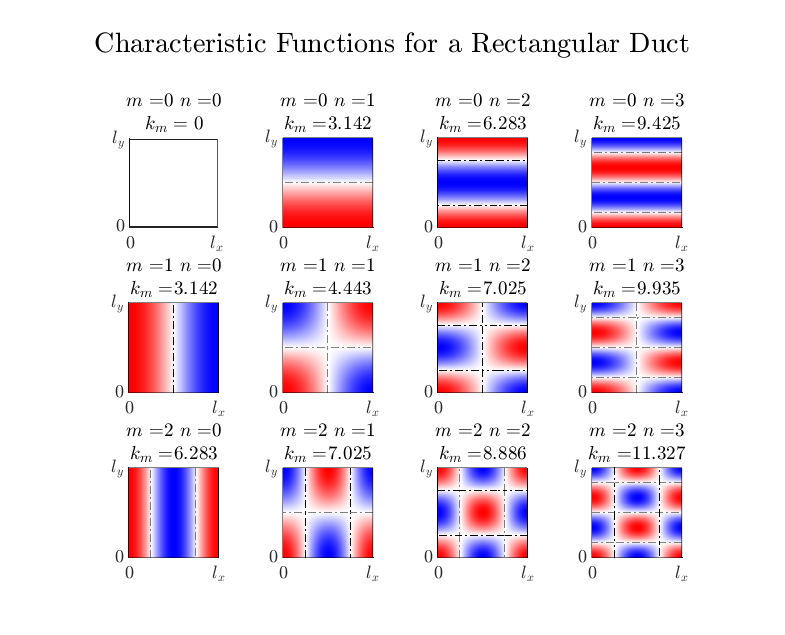
\includegraphics{../matlab/02_background/cross_section_rect.eps}
  \caption{Characteristic solutions to Equation \ref{eqn:02_wave_xy} with rigid wall in a rectangular cross-section where m=0:2 and n=0:3.  Nodal lines are depicted by the dot-dash lines.  The cross-sectional wave numbers, $k_m$, listed are for a duct of unit length and height.}
  \label{fig:02_cross_section_rect}
\end{figure}
The lines depicted in the figure are nodal lines and represent locations where there is zero pressure fluctuations for that acoustic mode.

The second set of known empirical solutions is for a circular cross-section with radius $R$,
\begin{equation}
  \Psi_{m,n}(r,\theta) = J_m(k_{mn}r)\exp\left\{\pm jm\theta\right\} \textrm{,}
  \label{eqn:02_psi_circ}
\end{equation}
where $J_m$ is the $m^\textrm{th}$ Bessel function of the first kind and the $\pm$ indicates the direction of spin.
If the left and right spin coefficients are equal in magnitude then a non-spinning mode is created.
In order to satisfy the solid wall boundary condition $J_m'(k_{mn}R) = 0$ which determines a set of discrete values for the cross-sectional wave number at the $n^\textrm{th}$ zero for the $m^\textrm{th}$ Bessel function.
Figure \ref{fig:02_cross_section_circ} shows the characteristic functions for a circular duct.
\begin{figure}
  \centering
  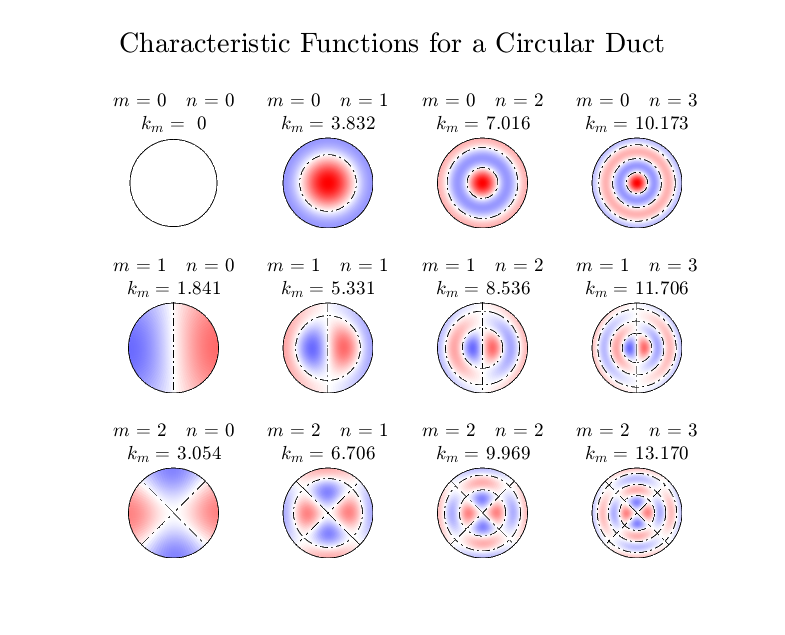
\includegraphics{../matlab/02_background/cross_section_circ.eps}
  \caption{Characteristic solutions to Equation \ref{eqn:02_wave_xy} with rigid wall in a circular cross-section where m=0:2 and n=0:3.  Nodal lines are depicted by the dot-dash lines.  The cross-sectional wave numbers, $k_m$, listed are for a duct of unit radius.}
  \label{fig:02_cross_section_circ}
\end{figure}
